\section{Tecnologia Implementata}
In questa sezione verranno illustrate le tecnologie implementate per la realizzazione del progetto
\subsection{NDEF e Sicurezza}
NDEF è un preciso standard per un formato di dati sui chip NFC, viene utilizzato in applicazioni quali le carde di credito, o gli smart poster, la struttura di un messaggio è quella vista nella seguente figura: 
\begin{center}
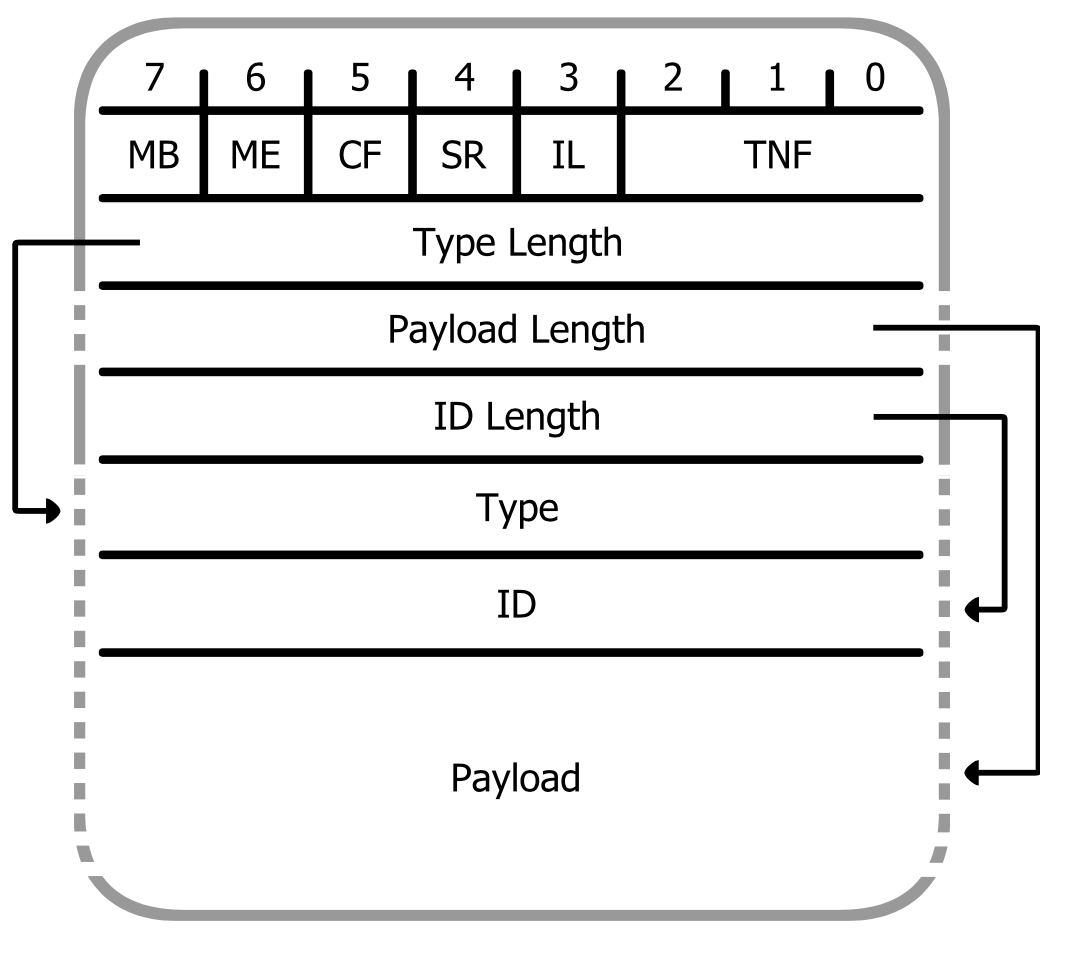
\includegraphics[scale=0.45]{ndefstructure}
\end{center}
In ordine abbiamo: 
\paragraph{Header}
\subparagraph{•}Message Begin (MB)
\subparagraph{•}Message End (ME)
\subparagraph{•}Chunk Flag (CF)
\subparagraph{•}Short record (SR)
\subparagraph{•}ID Length present (IL)
\subparagraph{•}Type Name Format (TNF)
\subparagraph{•}Length fields
\subparagraph{•}Type
\subparagraph{•}ID
\\I primi 5 parametri sono dei Flag, per finire invece abbiamo il \textbf{Payload} che è il messaggio.
\\Detto questo andiamo a concentrarci meglio su determinati campi quindi:
\paragraph{•}CF: indica il record che fa parte di una catena di record, quando il suo valore è pari a 1 vuol dire che c'è \textit{almeno} 1 altro record nella catena, invece quando non è settato vuol dire che ci troviamo o nel caso di record singolo o nel caso di ultimo elemento della catena. Una cosa da notare è che ME e CF non possono essere entrambi settati a 1
\paragraph{•}SR: quando viene messo ad 1 vuol dire che il record corrente è di tipologia short, questo comporta che il campo Payload Length, che si trova dentro Length fields, viene espresso tramite 1 byte, in alternativa viene espresso da 4 byte
\paragraph{•} IL: indica se nel record è presente un identificatore, se non dovesse essere abilitato questo comporta che non vi saranno il campo ID Length e il campo ID che è quello di identificazione del record.
\paragraph{•}TNF: serve per indicare la struttura del campo Type, è composto da 3 bit e può assumere solo i valori da 0 a 6 perché il numero 7 è riservato.
\\\\NDEF ha anche una firma
\begin{center}
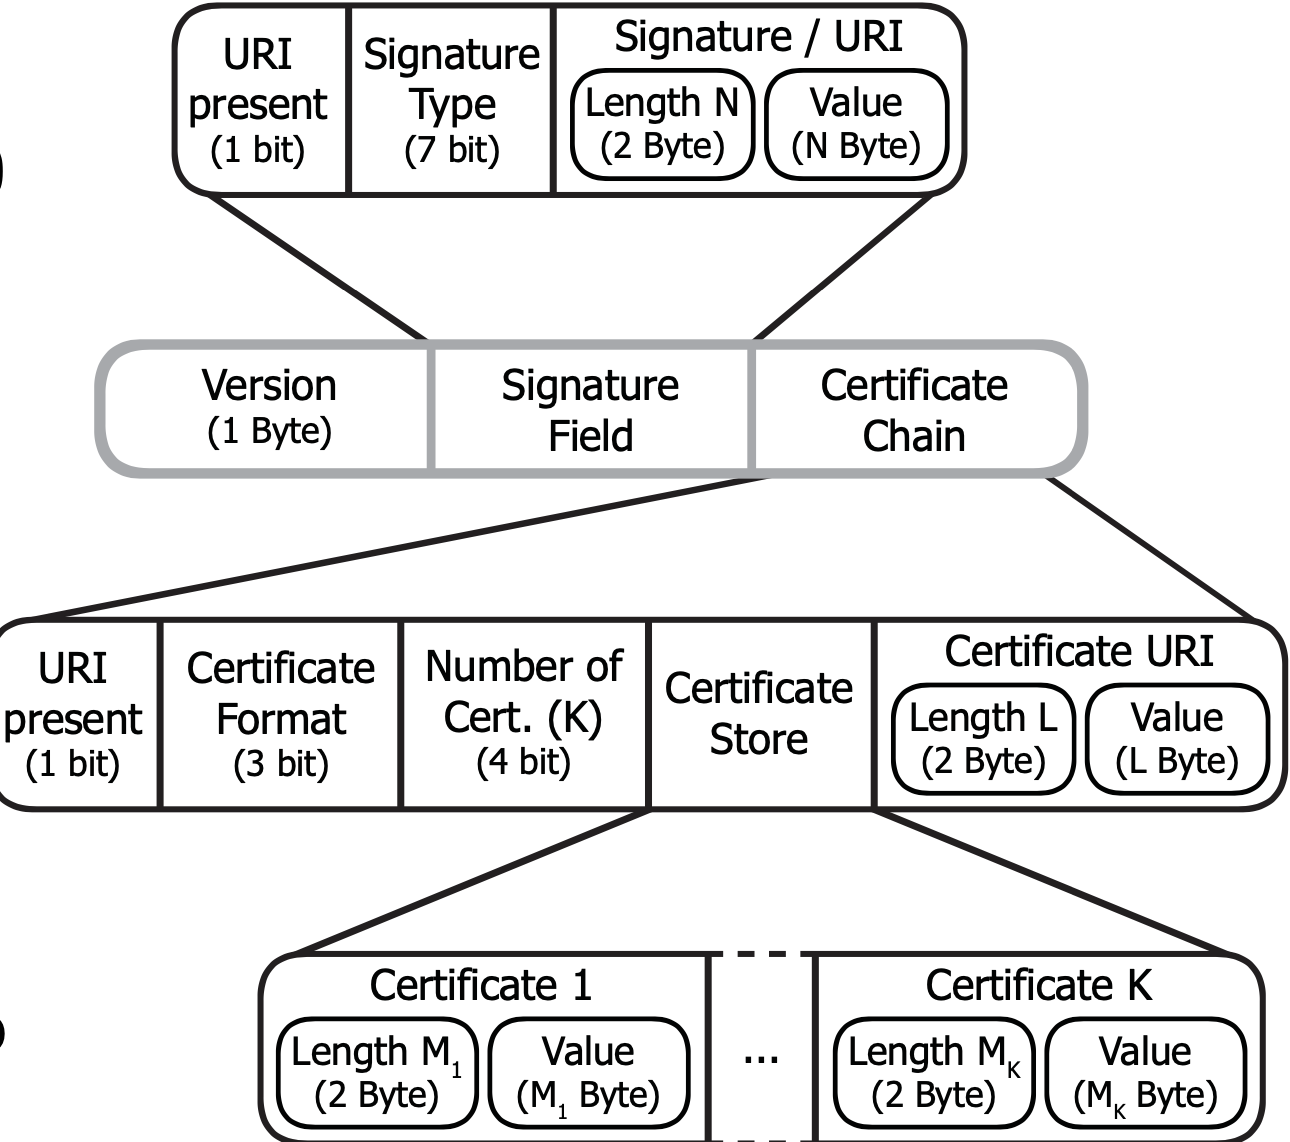
\includegraphics[scale=0.45]{ndefsign}
\end{center}
L'ultimo documento di specifica è stato rilasciato nel Novembre 2010, sostanzialmente ha una struttura fatta da un \textbf{campo firma}, che può essere una firma o una referenza URI ad una firma e da una \textbf{catena di certificati}, che è una catena di certificati PKI su un percorso sicuro.
\\Il record con la firma viene aggiunto ad una sequenza di record, e questo firma ogni record tra il record di firma appena precedente e se stesso, infatti un messaggio NDEF può contenere più di una firma.
\subsubsection{Cosa viene firmato?}
I campi che non vengono firmati sono MB/ME, questo perché se venissero firmati la firma non potrebbe essere agganciata al messaggio NDEF già firmato. Type, ID e Payload invece vanno firmati per assicurare l'integrità dei dati, mentre quando TNF viene cambiato, l'intero significato del record cambia, può essere quindi usato per nascondere dei record (identificati da type "Unknown"). 
\subsubsection{Sicurezza}
La tecnologia NFC è un'evoluzione dell'RFID, da un lato risulta meno predisposta ad attacchi esterni ma dall'altro lato è soggetta alle problematiche di sicurezza del suo predecessore. Le possibili minacce di sicurezza a cui sono sottoposti sono quelle riguardanti l'acquisizione, o l'alterazione dei dati contenuti nel tag, queste minacce possono avvenire mediante interrogazioni fraudolente o mediante intercettazione delle informazioni grazie a ricevitori radio durante la lettura da parte di un lettore autorizzato.
\subsubsection{Intercettazioni}
da fare
\subsubsection{Modifica dei dati}
da fare
\subsubsection{Man in the middle}
da fare
\subsection{Inserimento di falsi messaggi}
da fare
\subsection{NoSQL Database}
NoSQL è una tecnologia che promuove sistemi software dove la persistenza dei dati è in generale caratterizzata dal fatto di non utilizzare il modello relazionale. L'espressione "NoSQL" fa riferimento al linguaggio SQL, che è il più comune linguaggio di interrogazione dei dati nei database relazionali.
\\Questi archivi di dati il più delle volte non richiedono uno schema fisso (schemaless), evitano spesso le operazioni di giunzione (join) e puntano a scalare in modo orizzontale. Gli accademici e gli articoli si riferiscono a queste basi di dati come memorizzazione strutturata (structured storage). Per il progetto è stata utilizzata questa tecnologia per tenere in memoria fisica (tramite un file con estensione .txt) gli abbonamenti dei vari utenti
\subsection{WindowBuilder}
Per la realizzazione dell'interfaccia grafica in Java è stato usato il plug-in WIndowBuilder di Eclipse. Questo plug-in è composto a partire dalle liberire SWT Designer e Swing Designer e rende comoda e veloce la creazione di interfacce grafiche (GUI) per le applicazioni Java. Usando il WYSIWYG visual designer e gli strumenti di layout è possibile creare finestre complesse, e per ogni elemento messo verrà generato il codice contente la posizione dell'elemento e la sua dichiarazione.
\\Inoltre, il codice generato da questa libreria non richiede l'uso di altre librerie personalizzate per compilarlo ed eseguirlo, inoltre è possibile dall'interfaccia grafica creare eventi che poi andranno compilati mediante codice scritto in dei blocchi di \textit{ActionListener}, è possibile generare diversi tipi di eventi, dal click del mouse, alla pressione di un tasto sulla tastiera, o persino al movimento nella finestra del mouse.

\subsection{Cassandra}
Apache Cassandra è un DBMS distribuito e open source. Si tratta di un progetto Top-Level, sviluppato da Apache Software Foundation per gestire grandi quantità di dati dislocati in diversi server, fornendo un servizio orientato alla disponibilità.
\\È una soluzione NoSQL che inizialmente fu sviluppata da Facebook, un modello di dati simile a BigTable in esecuzione su un'infrastruttura tipi Amazon-Dynamo. Cassandra fornisce una struttura di memorizzazione chiave-valore, con Eventual Consistency.
\begin{center}
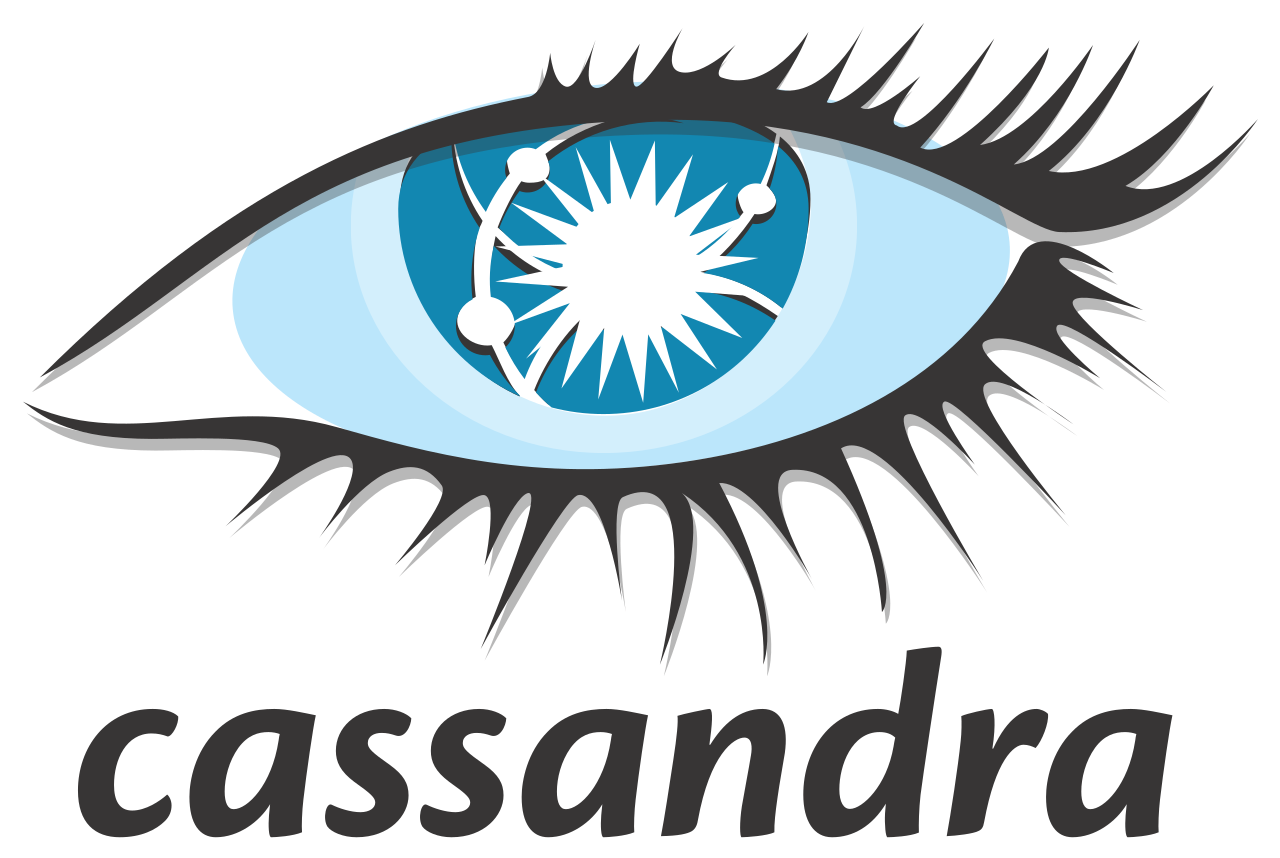
\includegraphics[scale=0.15]{cassandra}
\end{center}
Alle chiavi corrispondono dei valori, raggruppati in famiglie di colonne: una famiglia di colonne è definita quando il database viene creato. Tuttavia le colonne possono essere aggiunte a una famiglia in qualsiasi momento.
\\Le colonne sono aggiunte solo specificando le chiavi, così differenti chiavi possono avere differenti numeri di colonne in una data famiglia. I valori di una famiglia di colonne sono memorizzati insieme, questo perché Cassandra adotta un approccio ibrido tra DBMS orientato alle colonne e la memorizzazione orientata alle righe.
\\Come caratteristiche principali abbiamo:
\paragraph{•} Decentralizzazione: i nodi nel cluster sono identici, non c'è alcun single point of failure
\paragraph{•} Fault-tolerance: i dati vengono replicati in maniera automatica su più nodi, la replica è supportata tramite vari data center e la sostituzione dei nodi può avvenire senza downtime.
\paragraph{•} Tunable consistency: il livello di coerenza può essere modificato (da writes never fail a block for all replicas to be readable).
\paragraph{•} Elasticità: il throughput di lettura o scrittura scala linearmente con l'aggiunta di nuove macchine, senza downtime e senza interruzione di alcun applicativo.

\subsection{UUID}
\subsection{Crittografia}